\subsubsection{Presentation Layer}

Det første der blev opsat til kasseapparatet var grænsefladens view. Dette kan virke lidt bagvendt, men det var fra starten et fokus at skabe et anderledes kasseapparat der var nemt at benytte. Med dette menes der et program med en klar vej fra start til slut. Der måtte gerne være flere måder at gennemføre salg på, men brugeren måtte ikke være tvunget til at benytte sig af allesammen.
Som man kan se på figur \ref{fig:sub2} er kasseapparatet delt op i 3 segmenter. Her er idéen at produkterne skulle være i segmentet på venstre side, indkøbskurven i midten, og knapperne til brug i betalingen på højre side. Derved ville et salg gå fra venstre mod højre, i det at man først ville tilføje et produkt i venstre segment. Disse ville komme frem i det midterste segment, og til sidst ville betalingen blive gennemført i højre segment. 

\begin{figure}[H]
	\centering
	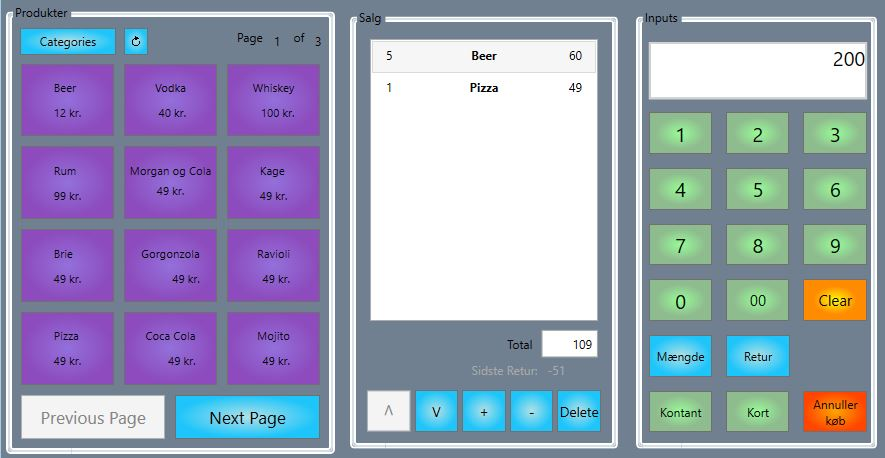
\includegraphics[width=0.9\linewidth]{Projektbeskrivelse/DesignOgImplementering/pics/GUI}
	\caption{Endelig Implementering}
	\label{fig:sub2}
\end{figure}

For at sikre at der var mange måder at tilføje produkter på, blev det udviklet så man kunne tilføje flere produkter, ved at klikke gentagne gange på hvert produkt. Denne funktionalitet virkede især smart, da kasseapparatet var tænkt til at skulle køre på en touch skærm. Samtidig kan man trykke på et tilføjet produkt i indkøbskurven, skrive et antal i betalingsdelen og trykke på mængde. Så vil det angivne antal af produktet blive tilføjet.\\

\textbf{Knapper og sideskift} \\
Noget der er lagt meget tid i er knappeskift. Dette blev implementeret ved at oprette et kontrolobjekt til knapper\footnote{ProductButtonControl klassen. Der kan læses mere om dette objekt i ProduktDokumentationen (indsæt sidetal samt figur nummer)}. Dette objekt indeholder en liste der inderholder liste af 12 knapper. Derved kan der nemt skiftes side af knapper bare ved at ændre index på den liste der vises på kasseapparatets produktknapper.